\section{Introduction}
\label{sec:introduction}

\stimfigcap-ground segregation is a concept that refers to the way the brain organizes visual information into distinct objects and backgrounds. This process allows us to perceive and understand the world by organizing complex visual stimuli into meaningful objects and backgrounds. In this process, the \stimfig{} is the object or part of the visual stimulus that is perceived as the main subject, while the ground is the surrounding context or background. Researchers in the field of perception have long been interested in understanding how the brain processes and organizes visual information through \stimfig-ground segregation \cite{Julesz1983, Julesz1984, Nothdurft1985a, Williams1992, Wagemans2012}.
Many studies have focused on the mechanisms underlying this process using visual texture stimuli. In particular, they investigated the role of a single feature, such as contrast, spatial frequency, color, orientation, or movement direction, in determining the difference between the \stimfig{} and background \cite{Hadjipapas2015, Bredfeldt2002, Henriksson2008, Shapley2011, Lamme1995}. Such an approach allows for simpler segregation than analyzing textures defined by multiple features \cite{Sagi1984, Treisman1980}.

The degree to which texture elements differ in a \stimfig{} and background affects the speed and accuracy of \stimfig-ground segregation \cite{Nothdurft1985a, Nothdurft1985b, Landy1991, Motoyoshi1999, Nothdurft1991a, Nothdurft1991b, DeWeerd1992}.
In particular, studies have shown that the extent of difference between elements on a specific dimension, as well as their relative proximity within the \stimfig, play a role in this process \cite{MaryamPLACEHOLDER}. Altering the \stimfig{} in these manners provides essential information to the neural mechanisms responsible for combining elements that make up that \stimfig{} and segregate it from the background. It has been proposed that these mechanisms are governed by the ability of the neuronal populations' oscillations in low-level visual areas to synchronize in the gamma frequency range \cite{Malsburg1995, Singer1995a, Gray1999}.

Brain oscillations are repetitive patterns of neural activity that can be observed in the brain. These patterns occur at different frequencies and have been linked to a range of mental states and cognitive processes \cite{BuzsakiBook2006:5}. Notably, gamma brain waves (25-80 Hz) are believed to be involved in perception \cite{Eckhorn1988, Gray1989, Kreiter1996, Livingstone1996, Fries1997, Gail2000}. The mechanisms that give rise to gamma oscillations are not well understood, but it is thought that they result from the synchronized activity of neurons in the brain \cite{Wang1996, Buzsaki2012, Fries2015}. This synchronization may be influenced by the interaction of inhibitory and excitatory neurons, as well as the action of neurotransmitters \cite{Fries2007, Tiesinga2009, Tiesinga2010}. 

Synchronization in networks of weakly coupled oscillators (WCOs) is influenced by two factors: the degree to which the intrinsic frequencies of the oscillators differ (detuning) and the strength of their coupling \cite{Pikovsky2002, Tiesinga2010, Lowet2015}. If the coupling strength is strong enough, the oscillators synchronize, with the critical value for synchronization depending on the detuning. The region of synchronization in the two-dimensional parameter space is referred to as \say{Arnold tongue} due to its triangular shape.
Neural computational models often depict local neuronal populations as oscillators, as they can produce gamma rhythms in response to local stimulation \cite{IzhikevichBook2004:9}. The strength of synchronization between them depends on the two characteristics mentioned above. The contrast between elements in a texture stimulus impacts the frequency detuning \cite{Lowet2017, Ray2010}, and the proximity of those elements affects the coupling strength \cite{Gilbert1983, Tso1986a, Lowet2015, Lowet2017, Stettler2002, MaryamPLACEHOLDER}. Hence, these parameters influence local synchronization between neurons, as confirmed by previous studies \cite{Lowet2017, MaryamPLACEHOLDER}. Section \ref{sec:twco} gives a more in-depth description of the effects of stimuli features on neural synchronization.

A recent study by Karimian has proposed a model of the visual cortex using Kuramoto oscillators and Gabor texture stimuli with varying contrast heterogeneity among texture elements and their coarseness \cite{MaryamPLACEHOLDER}, as shown in the examples in Figure \ref{fig:gabor-contrast-example}. In these textures, a \stimfig{} region was defined by less heterogeneous contrasts compared to the background.
They then used this model to evaluate the extent to which synchrony is predictive of human performance in a \stimfig-ground segregation experiment. The results showed that human \stimfig-ground segregation performance with the same stimuli conformed to model simulations. This suggests that synchrony of gamma oscillations is predictive of human performance in \stimfig-ground segregation. 

\begin{figure}[!htp]
    \centering
    \begin{subfigure}[t]{0.3\textwidth}
        \centering
        
\includegraphics[width=0.65\textwidth]{src/assets/images/25patches/dist-1.0000___contrast-0.0100.png}
        \caption{Low contrast heterogeneity and low coarseness.}
    \end{subfigure}
    \hspace{0.03\textwidth}
    \begin{subfigure}[t]{0.3\textwidth}
        \centering
        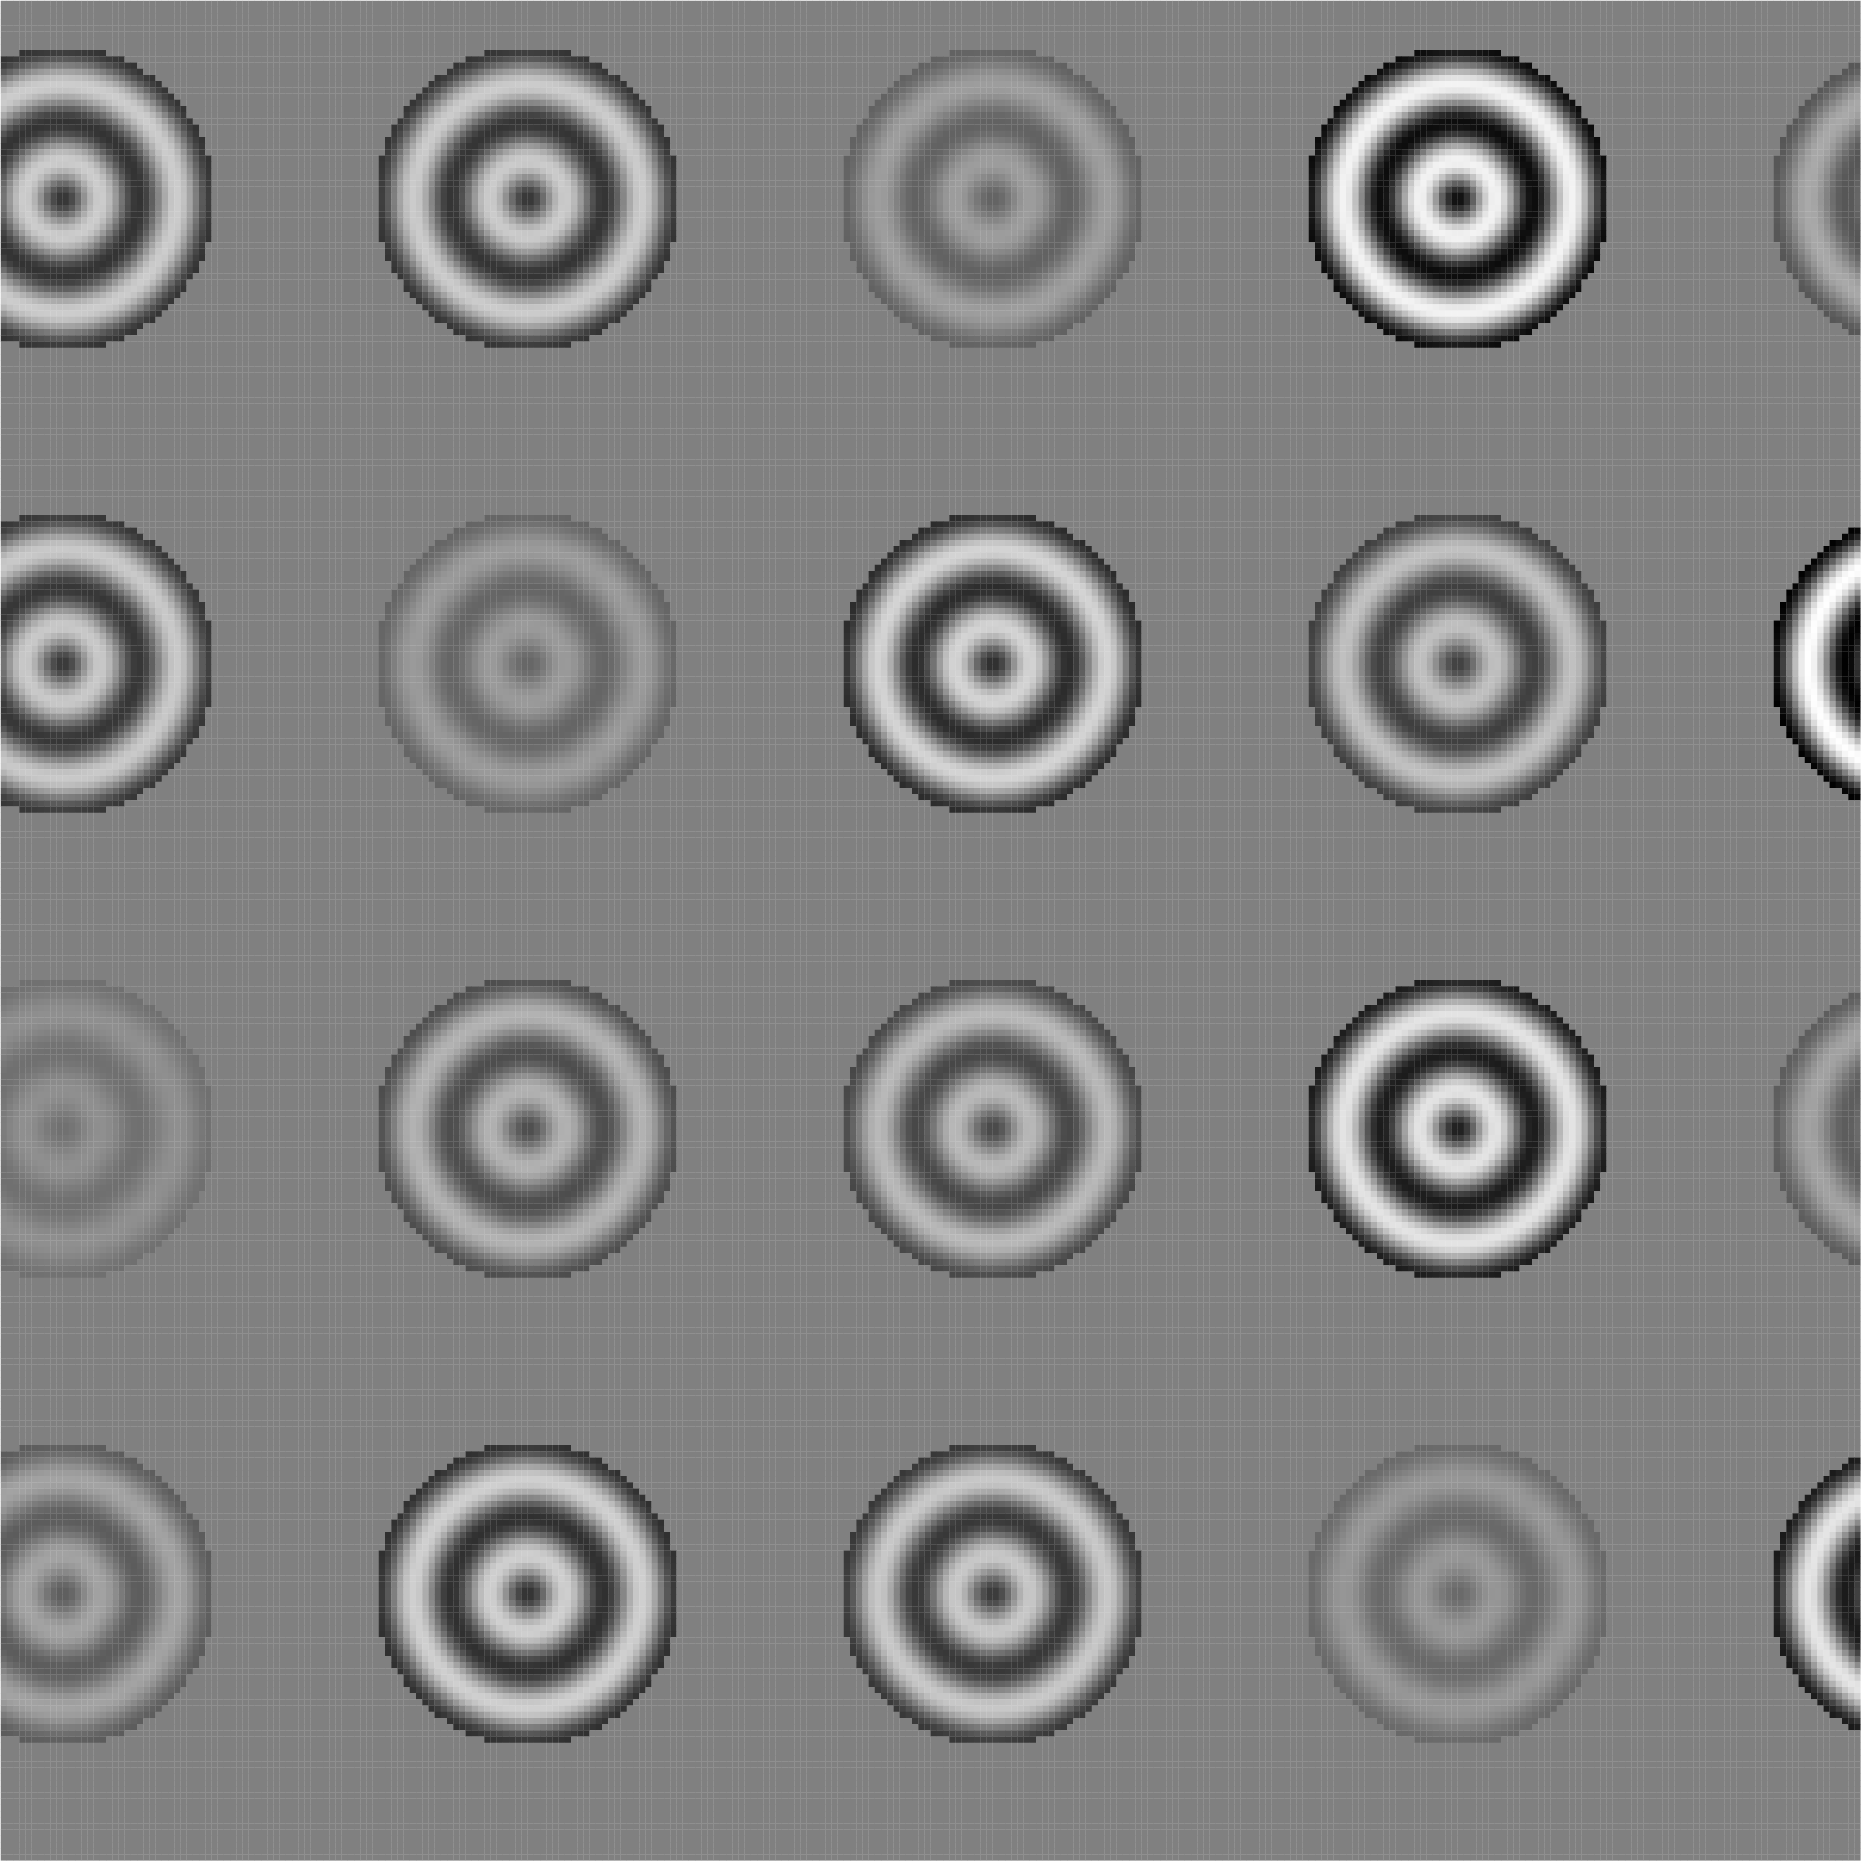
\includegraphics[width=0.65\textwidth]{src/assets/images/25patches/dist-1.5000___contrast-1.0000.png}
        \caption{High contrast heterogeneity and high coarseness.}
    \end{subfigure}
    \caption[Gabor stimuli examples]{Examples of a Gabor texture stimuli with varying contrast heterogeneity among texture elements and their coarseness.}
    \label{fig:gabor-contrast-example}
\end{figure}


The Pyramidal Interneuron Network Gamma (PING) model is a computational model that seeks to explain the origins of gamma oscillations in the brain. It proposes that these oscillations are generated by the interactions between two types of brain cells: pyramidal cells and interneurons \cite{Wilson1972, Whittington2000, Hansel2003}. Pyramidal cells are excitatory neurons that transmit signals to other brain regions, while interneurons are inhibitory neurons that help regulate the activity of pyramidal cells. The PING model focuses on the transmission of signals between these neurons. In contrast, the Kuramoto model focuses solely on the synchronization of oscillating units \cite{Breakspear2010}, such as the firing of neurons. This difference in focus means that the PING model is considered to be more biologically plausible, as it more accurately represents the complex interactions between neurons in the brain.

The present thesis uses the PING model to investigate the role of gamma oscillations in \stimfig-ground segregation. We evaluate the extent to which synchrony of gamma oscillations, as modeled by the PING network, is predictive of human performance in experiments conducted by Karimian \cite{MaryamPLACEHOLDER}. 
We imitate the behavior of neurons using the Izhikevich model, which has been shown to exhibit a wide range of computational properties, including the ability to generate gamma-band oscillations \cite{Izhikevich2003}. To use as an input to the model, we reconstruct the stimuli introduced by Karimian \cite{MaryamPLACEHOLDER}. We then present the results of neural synchronization in our own simulations. The results show that synchrony of gamma oscillations is predictive of human performance in \stimfig-ground segregation, consistent with previous research.

\paragraph{Applications}

Modeling \stimfig-ground segregation in the brain can provide insights into the underlying neural mechanisms and computational principles of this process. These insights can help us understand how the brain processes visual information and how it is affected by various factors.

One of the potential applications of modeling \stimfig-ground segregation is in aiding the development of Artificial Intelligence (AI) algorithms that can mimic human visual perception, such as image and video recognition, object detection, and scene understanding. Current state-of-the-art AI models often rely on deep learning techniques, which do not explicitly model figure-ground segregation and can struggle to identify and segment objects in complex or cluttered scenes accurately \cite{Chu2020}. As \stimfig-ground segregation neural models explicitly take into account the principles of visual perception, they have the potential to help the AI identify objects with higher accuracy.
Secondly, \stimfig-ground segregation models can be more data and computationally efficient than current state-of-the-art AI models, as they do not require large amounts of training data and can be applied to a wide range of visual scenes. Thus, if integrated into an AI model, these models can improve the time-to-solution and reduce the reliance on data.
Finally, neural perception models can provide a more interpretable and explainable representation of visual information, as they explicitly model the underlying computational principles. This can help better understand and interpret how these models work and how they can be improved.

Another conceivable application of figure-ground segregation models is in the study of visual disorders and dysfunctions. By understanding the neural mechanisms that regulate figure-ground segregation in the brain, researchers may be able to identify the underlying causes of visual disorders, such as amblyopia (lazy eye) or strabismus (crossed eyes), and develop more effective interventions and treatments for these conditions.

\begin{comment}
Additionally, visual perception models, such as \stimfig-ground segregation, could be applied to improve assistive technologies for individuals with visual impairments or disorders. For instance, it could be used in the development of new treatments for conditions that affect one's ability to focus and control their attention, such as dyslexia and ADHD. Potentially, these treatments could include visual exercises and therapies that are designed to improve \stimfig-ground segregation and, ultimately, the individual's ability to perceive and interpret visual information. Furthermore, \stimfig-ground segregation models could be used to design visual interfaces for everyday devices, such as phones, tablets, and computers, that are more intuitive and straightforward to use. For example, the design of buttons and menus could be optimized to make it easier for the visually impaired user to identify and select individual objects within the interface.

Besides the treatments for improving attention, figure-ground segregation models can be used to develop more effective training programs for tasks that require attention, such as piloting. Pilots must navigate complex environments, make rapid decisions, and manage multiple tasks while ignoring distractions. By using these models, visual simulations can be created to teach pilots to focus on important objects, such as other aircraft or obstacles, and ignore distractions. These simulations can be integrated into pilot training programs to improve their attention and decision-making abilities.
\end{comment}


\paragraph{Thesis organization}

The thesis is divided into several sections:
\begin{itemize}
    \item First, we provide an overview of the preliminary information helpful to understand the context of further sections. In particular, we provide the relevant background of visual processing in the brain, the neural action potential (spikes), and the theory of weakly coupled oscillators. This section is intended for readers who may not be familiar with the topics or with neuroscience in general.

    \item Then, we define the architecture of the model used in this thesis. Additionally, we describe the dynamics of the neurons and the composition of the input they receive.

    \item In the next section, we describe the process of constructing the texture stimuli used in the model and explain how these stimuli are translated into input for the neurons.

    \item Having defined the model, its architecture, and the external stimuli, we describe the evaluation of the model's simulations in terms of synchrony in the gamma range.

    \item Consequently, we present the results of our simulations and compare them to the results of behavioral experiments performed by Karimian \cite{MaryamPLACEHOLDER}. We use statistical analyses to evaluate the potential of our model to predict human behavior accurately.

    \item Finally, we summarize our findings and discuss the implications of our study.
\end{itemize}